\chapter{Planteamiento del Problema}

\section{Descripción de la Realidad Problemática}

En la última década, el crecimiento acelerado de los ecosistemas digitales ha transformado profundamente la manera en que se construye y percibe la opinión pública, especialmente en contextos electorales. Plataformas digitales como redes sociales, medios de comunicación en línea y servicios de contenido audiovisual han pasado a ser canales predominantes de información política, permitiendo a los ciudadanos expresar opiniones, consumir contenido y participar activamente en el debate público en tiempo real.

De acuerdo con \textcite{cr_digital2025}, más del 64\% de la población mundial utiliza redes sociales, lo que evidencia la masificación de estos entornos como espacios clave para la interacción social y política. Como se observa en la Figura \ref{fig:social_media_global}, este crecimiento ha consolidado a las plataformas digitales como un componente fundamental en la formación de la opinión pública contemporánea.

\begin{figure}[h]
	\begin{center}
		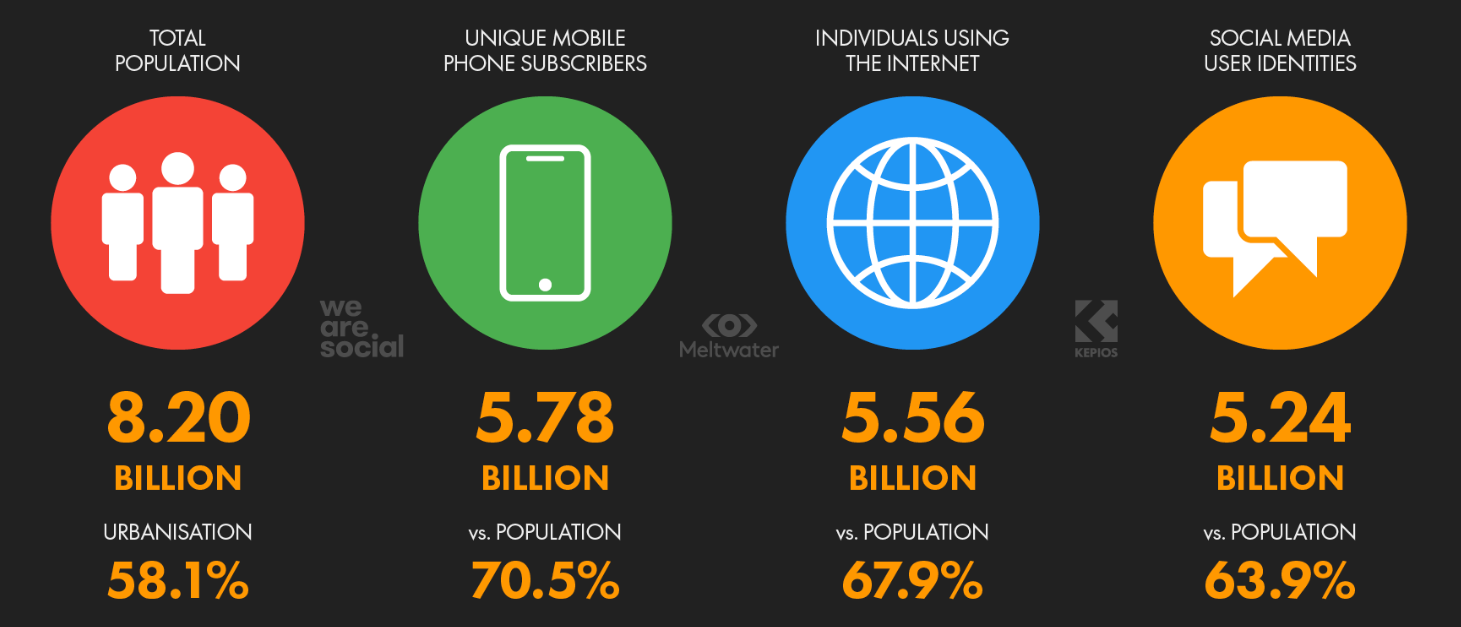
\includegraphics[width=0.7\textwidth]{1/figures/social_media_global.png}
		\caption[Uso global de redes sociales]{Uso global de redes sociales (2025).\\
		Fuente: \textcite{cr_digital2025}.}
		\label{fig:social_media_global}
	\end{center}
\end{figure}

En América Latina, esta tendencia es aún más pronunciada. Según el \textcite{cr_reuters2024}, aproximadamente el 70\% de los usuarios accede a noticias a través de redes sociales, lo que ha incrementado significativamente la influencia de estas plataformas en la formación de percepciones políticas. Tal como se aprecia en la Figura \ref{fig:news_social}, el consumo de información política en entornos digitales ha superado a los medios tradicionales en diversos segmentos de la población.

\begin{figure}[h]
	\begin{center}
		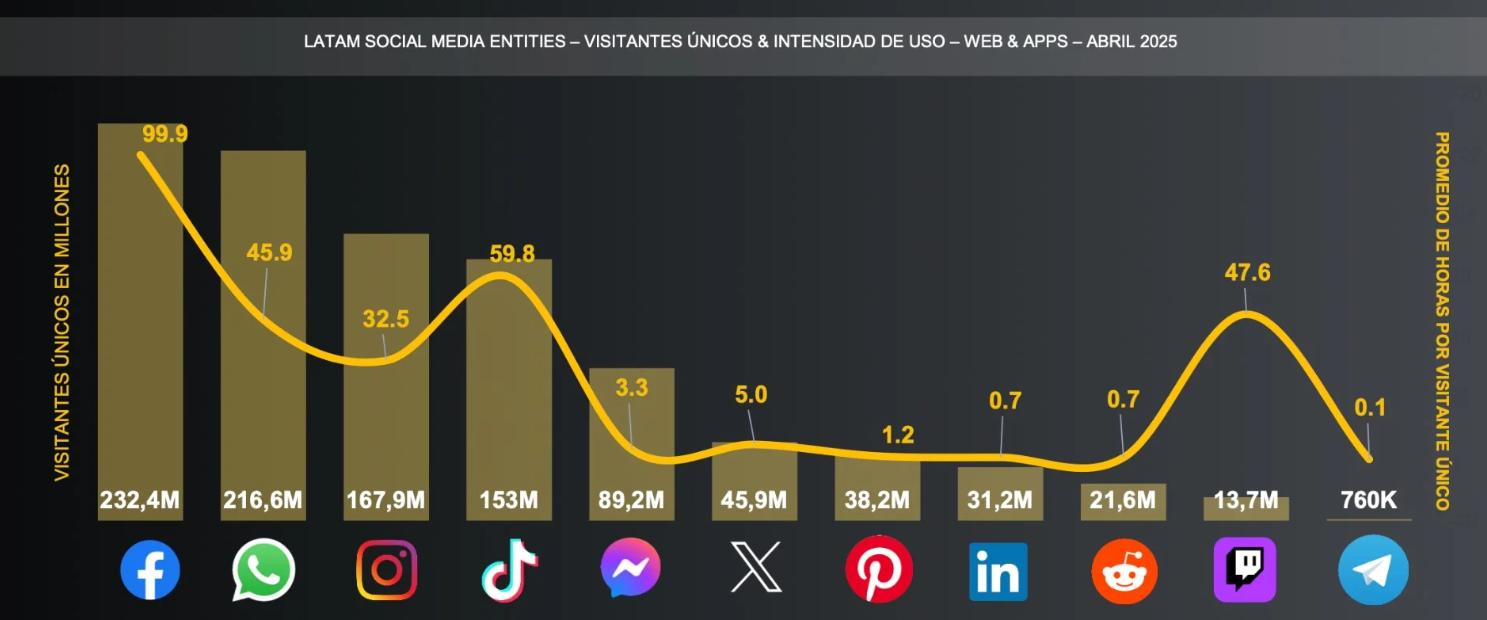
\includegraphics[width=0.7\textwidth]{1/figures/news_social_media.png}
		\caption[Consumo de noticias en redes sociales]{Consumo de noticias a través de redes sociales en América Latina.\\
		Fuente: \textcite{cr_reuters2024}.}
		\label{fig:news_social}
	\end{center}
\end{figure}

En el caso específico del Perú, el acceso a Internet ha alcanzado aproximadamente el 82\% de la población, lo que equivale a más de 28 millones de usuarios conectados, según el Instituto Nacional de Estadística e Informática \parencite{cr_inei2024}. Como se muestra en la Figura \ref{fig:internet_peru}, este alto nivel de penetración digital refuerza la relevancia de analizar la percepción pública en entornos digitales dentro del contexto nacional.

\begin{figure}[h]
	\begin{center}
		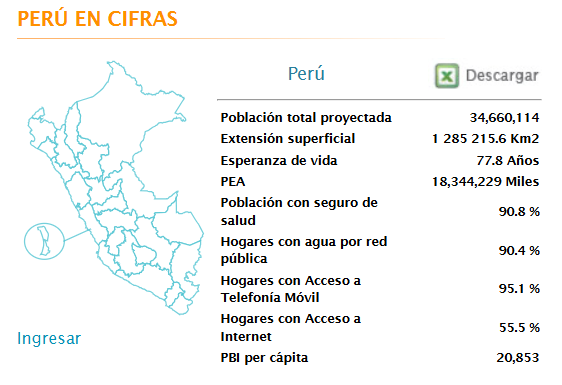
\includegraphics[width=0.65\textwidth]{1/figures/internet_peru.png}
		\caption[Usuarios de internet en Perú]{Acceso a Internet en Perú (2024).\\
		Fuente: \textcite{cr_inei2024}.}
		\label{fig:internet_peru}
	\end{center}
\end{figure}

Sin embargo, este crecimiento también ha generado nuevos desafíos. La sobrecarga informativa, la desinformación y la polarización dificultan la comprensión precisa de la percepción ciudadana en contextos electorales. Tal como señala \textcite{cr_castells2015comunicacion}, la comunicación digital ha dado lugar a una dinámica en la que los ciudadanos no solo consumen información, sino que también la reinterpretan y amplifican, generando múltiples capas de significado.

En este contexto, los métodos tradicionales de análisis de opinión pública, como encuestas o estudios cualitativos, presentan limitaciones importantes debido a su costo, baja frecuencia y limitada capacidad de capturar dinámicas en tiempo real. Por otro lado, los enfoques computacionales existentes suelen centrarse en una sola fuente de datos, como redes sociales, ignorando la diversidad de actores y formatos presentes en el ecosistema digital.

Asimismo, existe una brecha significativa entre el discurso mediático y la percepción ciudadana. Mientras los medios de comunicación establecen agendas informativas, los ciudadanos reaccionan de manera independiente en redes sociales, generando diferencias que no son adecuadamente modeladas por los enfoques actuales. Esta problemática resulta crítica durante procesos electorales, donde la identificación de tendencias, temas relevantes y cambios en la percepción pública es fundamental.

Por otro lado, el avance de los Modelos de Lenguaje de Gran Escala (LLMs) ha abierto nuevas oportunidades para el análisis semántico profundo de grandes volúmenes de datos. Según \textcite{cr_bommasani2021foundation}, estos modelos permiten capturar relaciones complejas en el lenguaje natural, superando las limitaciones de técnicas tradicionales de procesamiento de lenguaje natural.

En consecuencia, se identifica la necesidad de desarrollar un enfoque integral que permita analizar la percepción nacional en contextos electorales mediante la integración de múltiples fuentes de información, el uso de modelos avanzados de lenguaje y la representación estructurada de relaciones mediante grafos de conocimiento.

\section{Formulación del Problema}

\subsection{Problema General}
PG: \newcommand{\ProblemaGeneral}{
¿Es posible analizar la percepción nacional en contextos electorales mediante un sistema de Inteligencia Electoral basado en modelos de lenguaje de gran escala (LLMs), minería de sentimientos y detección dinámica de temas en ecosistemas digitales multi-fuente?
}
\ProblemaGeneral

\subsection{Problemas Específicos}

\newcommand{\Pbone}{¿Qué enfoques existen en la literatura para el análisis de opinión pública mediante inteligencia artificial?}
\newcommand{\Pbtwo}{¿Cómo integrar múltiples fuentes de datos (prensa, redes sociales y plataformas audiovisuales) para representar la percepción pública?}
\newcommand{\Pbthree}{¿Cuál es el impacto del uso de LLMs en el análisis de sentimientos y detección de temas?}
\newcommand{\Pbfour}{¿Cómo modelar las relaciones entre discurso mediático y percepción ciudadana mediante grafos de conocimiento?}

\begin{itemize}
	\item PE1: {\Pbone}
	\item PE2: {\Pbtwo}
	\item PE3: {\Pbthree}
	\item PE4: {\Pbfour}
\end{itemize}


\section{Objetivos de la Investigación}

\subsection{Objetivo General}
OG: \newcommand{\ObjetivoGeneral}{
Analizar la percepción nacional en contextos electorales mediante un sistema basado en LLMs, minería de sentimientos y detección de temas en ecosistemas digitales.
}
\ObjetivoGeneral
\subsection{Objetivos Específicos}

\newcommand{\Objone}{Analizar enfoques existentes en la literatura.}
\newcommand{\Objtwo}{Diseñar una arquitectura multi-fuente.}
\newcommand{\Objthree}{Evaluar el desempeño de LLMs en análisis de sentimientos y detección de temas.}
\newcommand{\Objfour}{Implementar un sistema basado en grafos de conocimiento y GraphRAG.}


\begin{itemize}
	\item OE1: {\Objone}
	\item OE2: {\Objtwo}
	\item OE3: {\Objthree}
	\item OE4: {\Objfour}
\end{itemize}

\section{Hipótesis}

\subsection{Hipótesis General}
HG: \newcommand{\HipotesisGeneral}{
El uso de modelos de lenguaje de gran escala (LLMs) permite analizar con mayor precisión la percepción nacional en entornos digitales multi-fuente durante contextos electorales.
}
\HipotesisGeneral
\subsection{Hipótesis Específicas}

\newcommand{\Hone}{La integración de múltiples fuentes de datos mejora la representatividad de la percepción pública.}
\newcommand{\Htwo}{Los modelos LLMs mejoran la precisión del análisis de sentimientos y detección de temas.}
\newcommand{\Hthree}{El uso de grafos de conocimiento permite modelar relaciones complejas entre actores y discursos.}
\newcommand{\Hfour}{El enfoque GraphRAG mejora la generación de insights en el análisis electoral.}

\begin{itemize}
	\item HE1: \Hone
	\item HE2: \Htwo
	\item HE3: \Hthree
	\item HE4: \Hfour
\end{itemize}


\section{Justificación de la Investigación}

\subsection{Teórica}

La presente investigación se justifica desde una perspectiva teórica debido a la necesidad de integrar enfoques contemporáneos en el análisis de la percepción pública dentro de ecosistemas digitales. Tradicionalmente, los estudios en análisis de opinión y comportamiento electoral se han apoyado en técnicas estadísticas clásicas y métodos de análisis de contenido manual o semiautomático. Sin embargo, el crecimiento exponencial de datos generados en redes sociales y plataformas digitales ha evidenciado limitaciones en dichos enfoques, especialmente en términos de escalabilidad, contextualización semántica y capacidad de adaptación en tiempo real.

En este contexto, el desarrollo de modelos de lenguaje de gran escala (LLMs) ha transformado significativamente el campo del Procesamiento de Lenguaje Natural (NLP), permitiendo una comprensión más profunda del lenguaje humano mediante representaciones contextuales avanzadas \parencite{pr_devlin2019bert, pr_brown2020gpt3}. A su vez, la minería de sentimientos ha evolucionado desde enfoques basados en lexicones hacia modelos más robustos que incorporan aprendizaje profundo, mejorando la precisión en la clasificación de opiniones y emociones \parencite{pr_pang2008opinion}.

Adicionalmente, la incorporación de grafos de conocimiento permite modelar relaciones semánticas complejas entre entidades, facilitando la interpretación estructurada de la información y el descubrimiento de patrones emergentes en grandes volúmenes de datos. En particular, enfoques recientes como GraphRAG combinan capacidades de recuperación de información con razonamiento basado en grafos, ampliando las posibilidades analíticas en sistemas inteligentes.

En este sentido, la presente investigación propone un enfoque integrador que articula LLMs, análisis de sentimientos, modelado de tópicos y grafos de conocimiento, contribuyendo a la literatura mediante una aproximación holística que supera las limitaciones de estudios previos centrados en técnicas aisladas. De esta manera, se aporta al desarrollo teórico de la inteligencia electoral como un campo emergente dentro de la analítica de datos y la ciencia política computacional.

\subsection{Práctica}

Desde el punto de vista práctico, la investigación responde a la creciente necesidad de comprender la percepción ciudadana en contextos electorales de manera oportuna, precisa y escalable. En la actualidad, los procesos electorales están fuertemente influenciados por la dinámica de los ecosistemas digitales, donde plataformas como redes sociales, medios digitales y foros en línea actúan como espacios clave para la formación de opinión pública.

El análisis tradicional de encuestas presenta limitaciones en términos de cobertura, costo y frecuencia de actualización, lo que dificulta capturar cambios dinámicos en la percepción ciudadana. En contraste, el uso de técnicas de minería de datos sobre información generada en tiempo real permite identificar tendencias emergentes, cambios en el sentimiento colectivo y temas de interés prioritario para la población.

En este contexto, la implementación de un sistema basado en LLMs y análisis multi-fuente permitirá procesar grandes volúmenes de datos provenientes de diversas plataformas digitales, generando indicadores relevantes sobre el comportamiento y percepción de los ciudadanos. Esto puede ser de utilidad para diversos actores, como analistas políticos, instituciones públicas, organizaciones de investigación y medios de comunicación, quienes podrán tomar decisiones más informadas basadas en evidencia empírica.

Asimismo, la capacidad de detección dinámica de temas relevantes permite identificar oportunamente eventos críticos, crisis de reputación o cambios en la agenda pública, contribuyendo a una mejor comprensión del entorno político y social.

\subsection{Metodológica}

En el ámbito metodológico, la investigación propone una arquitectura innovadora que integra múltiples técnicas avanzadas de análisis de datos, superando enfoques tradicionales basados en modelos únicos o fuentes de datos limitadas.

En primer lugar, se plantea un enfoque de análisis multi-fuente, que considera la integración de datos provenientes de diversas plataformas digitales, lo cual permite obtener una visión más completa y representativa del ecosistema informacional. En segundo lugar, se incorporan modelos de lenguaje de gran escala (LLMs) para el procesamiento semántico avanzado, facilitando tareas como clasificación de sentimientos, resumen de información y extracción de entidades.

Adicionalmente, se propone el uso de técnicas de modelado de tópicos para la detección automática de temas relevantes, permitiendo identificar patrones emergentes en el discurso público. Este componente se complementa con la construcción de grafos de conocimiento, los cuales modelan relaciones entre actores, temas y eventos, enriqueciendo el análisis con una dimensión estructural.

Finalmente, la integración de estos componentes mediante un enfoque tipo GraphRAG permite combinar capacidades de recuperación de información, razonamiento contextual y análisis estructurado, constituyendo una contribución metodológica significativa en el desarrollo de sistemas de inteligencia electoral basados en inteligencia artificial.

\section{Delimitación del Estudio}

\subsection{Espacial}

La investigación se delimita geográficamente al contexto peruano, con una extensión analítica hacia el ámbito latinoamericano. Esta delimitación responde a la relevancia de los procesos electorales en la región, caracterizados por una alta participación en entornos digitales y una creciente influencia de las redes sociales en la formación de opinión pública.

El enfoque en Perú permite contextualizar el análisis en un entorno específico con características sociopolíticas propias, mientras que la consideración del contexto latinoamericano posibilita la comparación y generalización de resultados en escenarios similares.

\subsection{Temporal}

En términos temporales, la investigación se centra en el análisis de datos recientes provenientes de ecosistemas digitales, priorizando información generada en los últimos años. Esta delimitación permite capturar dinámicas actuales en el comportamiento de los usuarios, así como tendencias emergentes en el uso de plataformas digitales para la expresión de opiniones políticas.

Asimismo, el enfoque en datos recientes es coherente con la naturaleza cambiante del entorno digital, donde los temas de interés y el sentimiento colectivo pueden variar rápidamente en función de eventos coyunturales.

\subsection{Conceptual}

Desde el punto de vista conceptual, la investigación se enfoca en el análisis de la percepción pública mediante técnicas de Procesamiento de Lenguaje Natural (NLP), modelos de lenguaje de gran escala (LLMs) y grafos de conocimiento.

Se consideran conceptos clave como minería de sentimientos, detección de tópicos, análisis semántico y modelado de relaciones entre entidades. Asimismo, se enmarca dentro del campo de la analítica de datos aplicada a la ciencia política, particularmente en el ámbito de la inteligencia electoral.

No se abordan aspectos relacionados con la predicción directa de resultados electorales, sino que el énfasis se encuentra en la comprensión de la percepción ciudadana y la identificación de patrones en el discurso público digital.